\subsection{Scenario 2}

\subsubsection{Configuration}

Ouvrir la page à l'adresse \url{http://}[adresse IP du contrôleur]\url{:8181/onos/ui/index.html#/topo}.
Pour voir ce qui se passe au niveau du contrôleur, on pourra si on le souhaite lancer une session wireshark sur l'interface concernée afin d'examiner les divers paquets Openflow transitant entre ONOS et switchs (notamment les paquets LLDP encapsulés en PACKET\_IN). Le filtre "tcp.port == 6633 \&\& openflow\_v4 \&\& (openflow\_v4.type == OFPT\_PACKET\_IN or openflow\_v4.type == OFPT\_PACKET\_OUT)" peut être utilisé pour supprimer les paquets inutiles.
Exécuter les instructions suivantes dans la console Mininet après avoir lancé le fichier general\_topology.py :

\begin{minted}{bash}
$ sudo ./general_topology.py [addresse IP du contrôleur]
$> h5 python scenario2/lldp_exploit.py 1 h5-eth0 &
$> h5 python scenario2/lldp_exploit.py 4 h5-eth0 &
$> h2 ping h11
\end{minted}

Attendre quelques secondes, puis arrêter le ping. Pour être certain que l'attaque fonctionne, on pourra faire le test suivant (ping entre h2 et h9).

\begin{minted}{bash}
$> h2 ping h9
\end{minted}


\subsubsection{Résultat}

\begin{figure}[h]
  	\centering
  	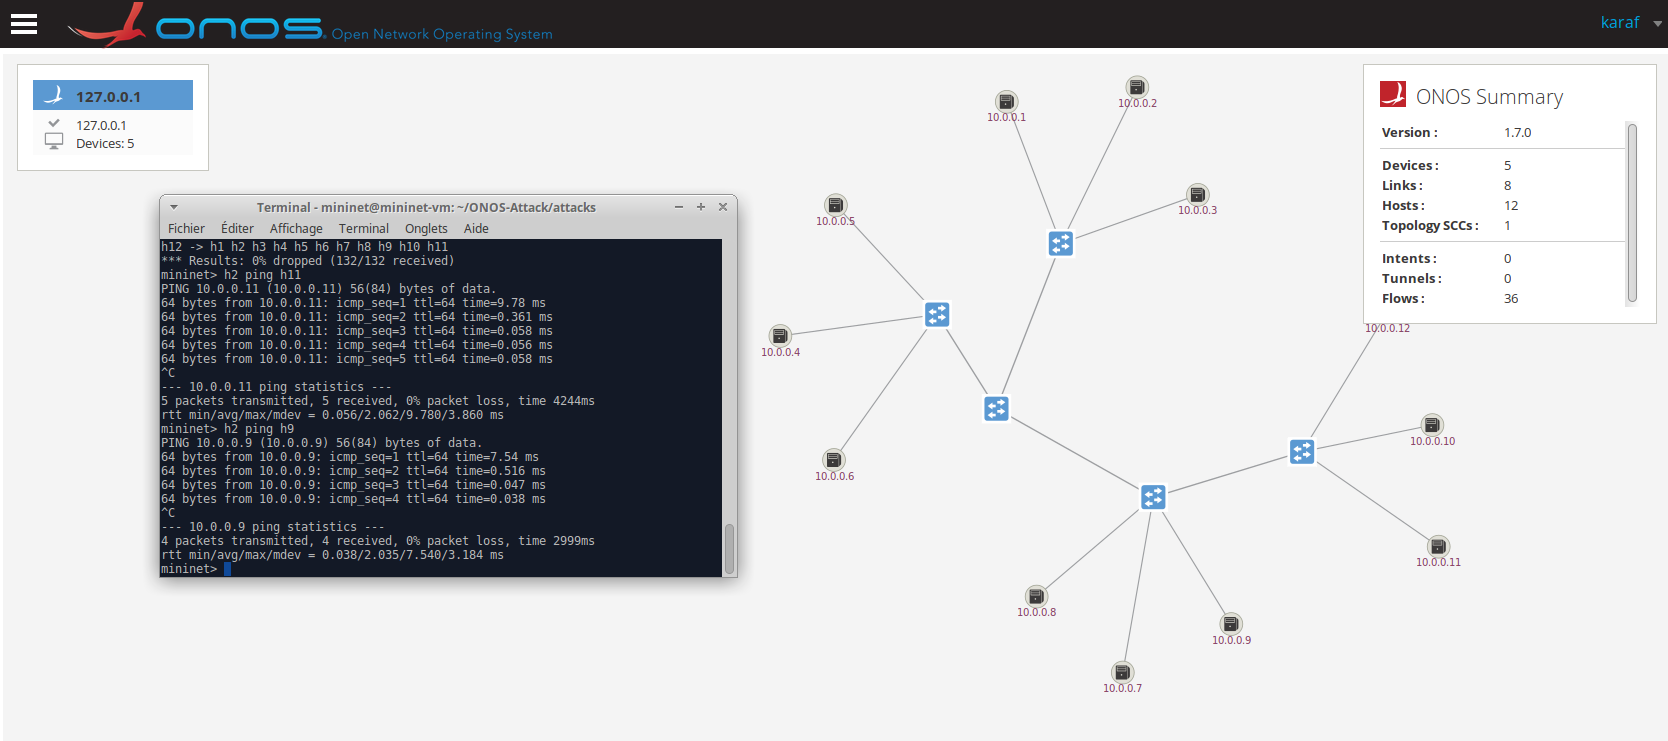
\includegraphics[width=1\textwidth]{scenario2_no_attack.png}
  	\caption{Cas normal : ping entre h2 et h11 possible}
\end{figure}


On observe alors la création de 2 nouveaux liens virtuels entre s1 et s2 et entre s2 et s4 qui n'existent pas dans la pratique (le résultat sur l'interface graphique est très parlant). Cela aboutit à l'impossibilité pour h2 de ping h11 puisque le chemin le plus court passe par le faux lien qui n'existe pas. Le ping entre h2 et h9 est en revanche toujours possible car le chemin le plus court reliant les 2 switchs ne passe pas par notre faux lien.\\

\begin{figure}[h]
  	\centering
  	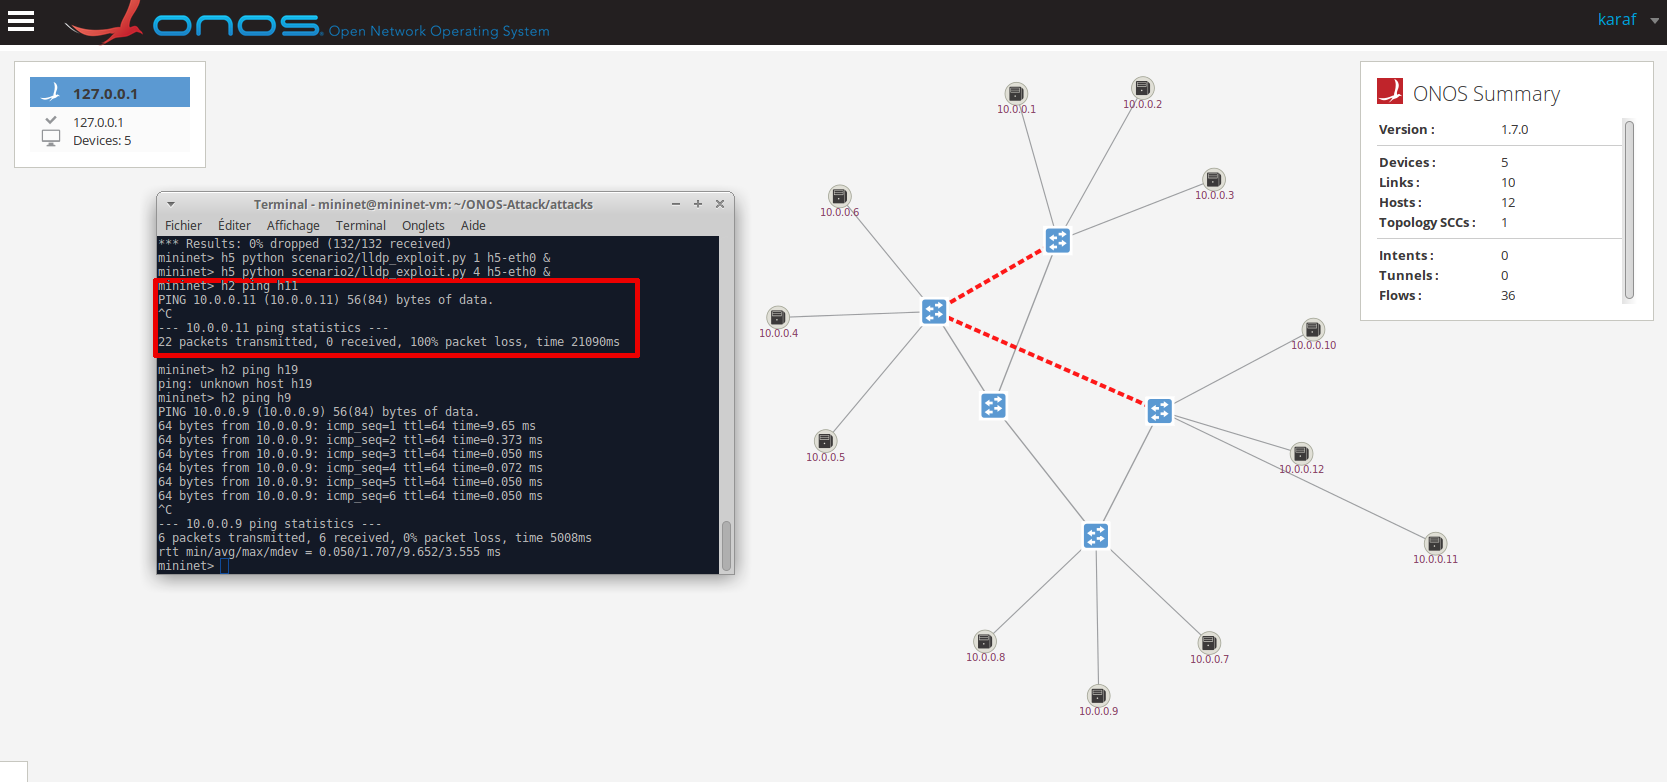
\includegraphics[width=1\textwidth]{scenario2_success_colored.png}
  	\caption{Réseau attaqué : ping entre h2 et h11 impossible}
\end{figure}

\underline{Conclusion :}\\
L'attaque est complexe à arrêter dans le cas d'un équipement malveillant directement présent sur le réseau. En effet, même si le contrôleur rajoute un champ signé dans les paquets LLDP qu'il envoie (afin de ne considérer à la réception que ceux dont il est à l'origine), si notre équipement malveillant arrive à récupérer un de ces paquets, il peut le rejouer et ainsi effectuer l'attaque, même si il ne peut plus réellement choisir les switchs à cibler. De toute façon aucun mécanisme semblable n'existe à l'heure actuelle sur ONOS par défaut et dans les applications installées.\\
L'attaque peut également être détournée en une attaque par homme au milieu si à la place de créer un faux lien on crée un lien vers un équipement qu'on contrôle, qui pourra se charger de rediriger le trafic après l'avoir intercepté. C'est un Man in the Middle plus puissant que dans la précédente attaque dans la mesure où c'est moins facilement détectable par le contrôleur.
